\chapter[$\zmod{2}$ Homology]{Simplicial $\ZZ_2$-Homology: Physical Algebra}
\section{Intro}
This chapter, we'll talk about \emph{homology}, which captures holes in a much
more satisfying way than higher homotopy groups do.
\begin{adjustwidth}{1.5em}{}
  \begin{remark}
    Although not exactly accurate, a good way to start to understand homology for
    a space $X$ is to view an $n$-manifold in $X$ that is not the boundary of an
    $(n+1)$-manifold-with-boundary as capturing some geometry of $X$ while an
    $n$-manifold that is the boundary of an $(n+1)$-dimensional
    manifold-with-boundary is not detecting any hole or structure.
  \end{remark}
\end{adjustwidth}
\section{Chains, Cycles, Boundaries, and the Homology Groups}
\begin{definition}
  An \emph{$n$-chain} of $K$ is a finite formal sum
  \[
    \sum_{i=1}^k \sigma_i
  \]
  of distinct $n$-simplices in $K$. Note that the dimensions of the simplices
  must be the same. So \emph{chain} will mean $n$-chain whenever the dimension
  is either unimportant or understood.
\end{definition}
\begin{definition}
  The \emph{$n$-chain group of $K$} (with coefficients in $\zmod{2}$), denoted
  $\mathsf{C}_n(K)$, is the collection of $n$-chains in $K$ under formal
  addition modulo 2. If there are no $n$-simplices in $K$, the $n$-chain group
  of $K$ is defined to be trivial (containing the ``empty'' chain).
\end{definition}
\begin{problem}[16.1]
  Check that $\msf C_n(K)$ is an abelian group.
\end{problem}
\begin{solution}
  \begin{enumerate}[label=(\arabic*)]
    \item $\epsilon = \sum_{i \in \varnothing} \sigma_i$.
    \item Associativity inherited from $\cup$.
    \item Closure inherited from $\cup$ over the domain given.
    \item Existence of inverses --- since we're taking formal linear
      combinations over $\zmod{2}$, then every element is its own inverse.
  \end{enumerate}
  Finally, to see that $\msf C_n(K)$ is abelian, observe that $+$ in $\msf
  C_n(K)$ inherits commutativity from $\cup$.
\end{solution}
\begin{definition}
  The \emph{$\zmod{2}$-boundary of an $n$-simplex $\sigma = \simp{n}$} is
  defined by
  \[
    \partial \sigma = \sum_{i=0}^n \simpdel{i}{n}
  \]
  the formal sum of the $(n-1)$-faces of $\sigma$.

  For a 0-simplex, the $\zmod{2}$ boundary is defined to be $0 \in \msf
  C_{-1}(K)$.
\end{definition}
\begin{definition}
  The \emph{$\zmod{2}$ boundary of an $n$-chain} is the sum of the boundaries of
  the simplices. That is, $\partial_n : \msf C_n(K) \to \msf C_{n-1}(K)$ is
  given by
  \[
    \partial\pn{\sum_{i=1}^k \sigma_i} = \sum_{i=1}^k \partial(\sigma_i)
  \]
\end{definition}
\begin{problem}[16.2]
  Verify that $\partial$ is a homomorphism, and use the definition to compute
  the $\zmod{2}$ boundary of $\sigma_1 + \sigma_2$ in Figure 16.1
\end{problem}
\begin{solution}
  We want to show $\partial$ is a homomorphism.
  \begin{enumerate}
    \item Let $\epsilon_n \in \msf C_n(K)$ be identity. We want to show
      $\partial(\epsilon_n) = \epsilon_{n-1}$. Taking the empty sum to be
      identity, we see
      \begin{align*}
        \partial(\epsilon_n)
        &=
        \partial\pn{\sum_{i\in \varnothing} \sigma_i} \\
        &= \sum_{i\in\varnothing} \partial\pn{\sigma_i} \\
        &= \epsilon_{n-1}
      \end{align*}
      as desired.
    \item That $\partial$ respects addition is definitional.
  \end{enumerate}
  We have $\partial(\sigma_1 + \sigma_2) = e_1 + e_2 + e_4 + e_5$.
\end{solution}
\begin{definition}
  An \emph{$n$-cycle} is an $n$-chain of $K$ whose boundary is zero. The set of
  all $n$-cycles on $K$ is denoted $\msf Z_n(K)$. An \emph{$n$-boundary} is an
  $n$-chain that is the boundary of an $(n+1)$-chain of $K$. The set of all
  $n$-boundaries is denoted $\msf B_n(K)$.
\end{definition}
% \begin{problem}[16.3]

% \end{problem}
\begin{problem}[16.4]
  Both $\msf Z_n(K)$ and $\msf B_n(K)$ are subgroups of $\msf C_n(K)$. Moreover,
  \[
    \partial \circ \partial = 0.
  \]
  In other words, $\partial_n \circ \partial_{n+1} = 0$ for each index $n \geq
  0$. Hence, $\msf B_n(K) \subset \msf Z_n(K)$.
\end{problem}
\begin{solution}
  Let $\sigma_1, \sigma_2 \in \msf Z_n(K)$. Then by linearity of $\partial_n$,
  we have
  \begin{align*}
    \partial_n(\sigma_1 + \sigma_2)
    &= \partial_n(\sigma_1) + \partial_n(\sigma_2) \\
    &= 0
  \end{align*}
  and hence $\msf Z_n(K) < \msf C_n(K)$.

  Now, let $\sigma_1, \sigma_2 \in \msf B_n(K)$. Then $\exists \tau_1, \tau_2
  \in \msf Z_{n+1}(K)$ such that $\partial_{n+1}(\tau_1) = \sigma_1,
  \partial_{n+1}(\tau_2) = \sigma_{2}$. Since $\msf Z_{n+1}(K) < \msf
  C_{n+1}(K)$, then $\tau_1 + \tau_2 \in \msf Z_{n+1}(K)$. Now, by linearity of
  $\partial$, we have
  \begin{align*}
    \partial_{n+1}(\tau_1 + \tau_2)
    &= \partial_{n+1}(\tau_1) + \partial_{n+1}(\tau_2) \\
    &= \sigma_1 + \sigma_2
  \end{align*}
  hence $\msf B_n(K)$ is a subset closed under the operation, so we have $\msf
  B_n(K) < \msf C_n(K)$.
\end{solution}
\begin{definition}
  Two $n$-cycles $\alpha$ and $\beta$ in $K$ are \emph{equivalent} or
  \emph{homologous} iff $\alpha-\beta = \partial(\gamma)$ for some $(n+1)$-chain
  $\gamma$. In other words, $\alpha$ and $\beta$ are homologous iff they differ
  by an element of the subgroup $\msf B_n(K)$, denoted by
  \[
    \alpha \sim_{\zmod{2}} \beta.
  \]
  The equivalence class of $\alpha$ is denoted by enclosing it in brackets
  thusly: $[\alpha]$. For $\zmod{2}$ $n$-chains, observe that $\alpha - \beta =
  \alpha + \beta$. So we see that two $n$-cycles are equivalent if together they
  bound an $(n+1)$-chain.
\end{definition}
\begin{problem}[16.5]
  List all the equivalence classes of $0$-cycles, 1-cycles, and 2-cycles in the
  complex in Figure 16.1.
\end{problem}
\begin{solution}
  {\color{red} maybe the next exercise will be more informative.}
\end{solution}
\begin{definition}
  The \emph{$n$\textsuperscript{th}-homology group} (with coefficients in
  $\zmod{2}$) of a finite simplicial complex $K$, denoted $\msf H_n(K)$, is the
  additive group whose elements are equivalence classes of cycles under the
  $\zmod{2}$-equivalence defined above, with $\bk{\alpha} + \bk{\beta} =
  \bk{\alpha +\beta}$. I.e.,
  \[
    \msf H_n(K) = \msf Z_n(K)/\msf B_n(K)
  \]
\end{definition}
\begin{problem}[F1]
  Consider the simplicial complex given below in Figure \ref{fig:F1}. Then for
  $n = 0, 1, 2$,
  \begin{enumerate}
    \item describe elements of $\msf C_n(K)$,
    \item compute $\msf Z_n(K)$,
    \item compute $\msf B_n(K)$, and
    \item compute $\msf H_n(K)$.
  \end{enumerate}
\end{problem}
\begin{figure}[H]
  \centering
  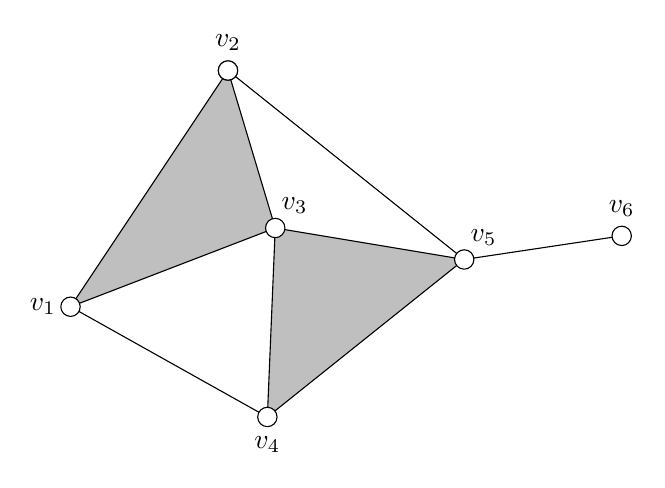
\begin{tikzpicture}[
      every node/.style={
        circle,
        draw=black,
        fill=white,
        inner sep=0pt,
        minimum size=7pt
      }
    ]

    \coordinate (v1) at (0,0);
    \coordinate (v2) at (2,3);
    \coordinate (v3) at (2.6,1);
    \coordinate (v4) at (2.5,-1.4);
    \coordinate (v5) at (5,.6);
    \coordinate (v6) at (7,.9);

    \draw[fill=gray!50!white] (v1) -- (v2) -- (v3) -- (v1) -- cycle;
    \draw[fill=gray!50!white] (v3) -- (v4) -- (v5) -- (v3) -- cycle;

    \draw (v1) -- (v4);
    \draw (v2) -- (v5);
    \draw (v5) -- (v6);

    \node (wv1) at (v1) {};
    \node (wv2) at (v2) {};
    \node (vv2) at (v2) {};
    \node (vv3) at (v3) {};
    \node (vv4) at (v4) {};
    \node (vv5) at (v5) {};
    \node (vv6) at (v6) {};

    \node[draw=none, xshift=-1em] (wv1) at (v1) {$v_1$};
    \node[draw=none, yshift=1em] (wv2) at (v2) {$v_2$};
    \node[draw=none, xshift=.7em, yshift=.8em] (wv3) at (v3) {$v_3$};
    \node[draw=none, yshift=-1em] (wv4) at (v4) {$v_4$};
    \node[draw=none, xshift=.7em, yshift=.8em] (wv5) at (v5) {$v_5$};
    \node[draw=none, yshift=1em] (wv6) at (v6) {$v_6$};
  \end{tikzpicture}
  \caption{Simplicial complex $K$}
  \label{fig:F1}
\end{figure}
\begin{solution}
  First, we redraw the simplicial complex as follows:
  \begin{figure}[H]
    \centering
    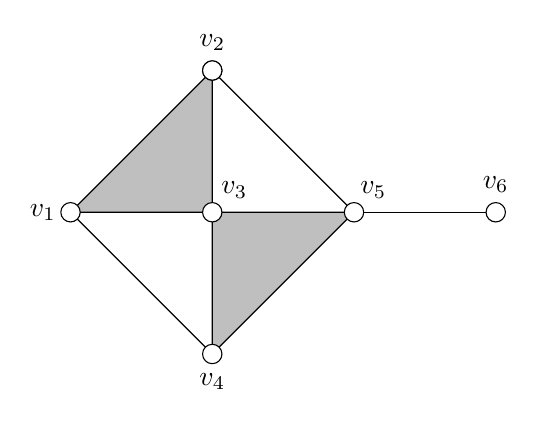
\begin{tikzpicture}[
        scale = .6,
        every node/.style={
          circle,
          draw=black,
          fill=white,
          inner sep=0pt,
          minimum size=7pt
        }
      ]

      \coordinate (v1) at (-3,0);
      \coordinate (v2) at (0,3);
      \coordinate (v3) at (0,0);
      \coordinate (v4) at (0,-3);
      \coordinate (v5) at (3,0);
      \coordinate (v6) at (6,0);

      \draw[fill=gray!50!white] (v1) -- (v2) -- (v3) -- (v1) -- cycle;
      \draw[fill=gray!50!white] (v3) -- (v4) -- (v5) -- (v3) -- cycle;

      \draw (v1) -- (v4);
      \draw (v2) -- (v5);
      \draw (v5) -- (v6);

      \node (wv1) at (v1) {};
      \node (wv2) at (v2) {};
      \node (vv2) at (v2) {};
      \node (vv3) at (v3) {};
      \node (vv4) at (v4) {};
      \node (vv5) at (v5) {};
      \node (vv6) at (v6) {};

      \node[draw=none, xshift=-1em] (wv1) at (v1) {$v_1$};
      \node[draw=none, yshift=1em] (wv2) at (v2) {$v_2$};
      \node[draw=none, xshift=.8em, yshift=.8em] (wv3) at (v3) {$v_3$};
      \node[draw=none, yshift=-1em] (wv4) at (v4) {$v_4$};
      \node[draw=none, xshift=.7em, yshift=.8em] (wv5) at (v5) {$v_5$};
      \node[draw=none, yshift=1em] (wv6) at (v6) {$v_6$};
    \end{tikzpicture}
    \caption{Simplicial complex $K$, straightened out}
  \end{figure}
  For the purposes of this problem, take angled brackets indicate span. We have
  \begin{enumerate}[label=(\roman*)]
    \item We calculate the $k=0$ case.
      \begin{enumerate}
        \item Elements of $\msf C_0(K)$ are formal linear combinations over the
          set $\set{v_1, v_2, \ldots, v_6}$. Then
          \[
            \msf C_0(K) = \ip[Big]{v_1, v_2, v_3, v_4, v_5, v_6}
          \]
          that is, collections of points in $\msf C_0(K)$.
        \item Let $\sigma_1, \ldots, \sigma_k \in \msf C_0(K).$ Then by definition,
          \begin{align*}
            \partial\pn{\sum_{i=1}^k \sigma_i}
            &= \sum_{i=1}^k \partial(\sigma_i)\\
            &= \sum_{i=1}^k 0 \\
            &= 0
          \end{align*}
          hence $\msf Z_n(K) = \msf C_n(K)$.
        \item A $\sigma \in \msf C_0(K)$ is an $n$-boundary if $\exists \tau \in
          \msf C_{1}(K)$ with $\partial(\tau) = \sigma$. Note, for any
          $1$-dimensional face $\set{v_iv_j} \in K$,
          \begin{align*}
            \partial(\set{v_iv_j})
            &= \set{v_i \widehat{v_j}} + \set{\widehat{v_i}v_j} \\
            &= \set{v_i} + \set{v_j} \\
            &= \delta_{ij}.
          \end{align*}
          Hence, any edge formed of a pair of two distinct vertices yields a
          nonempty boundary. Hence, we first count all edges:
          \begin{figure}[H]
            \centering
            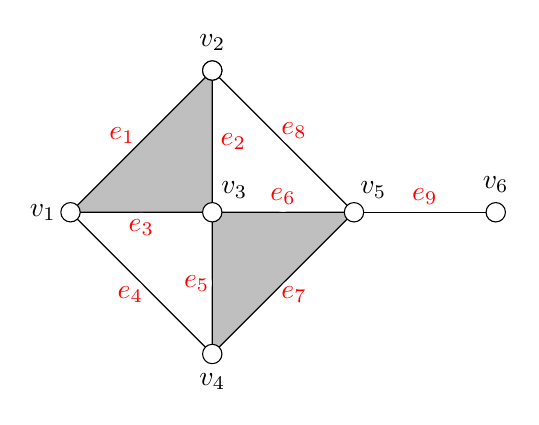
\begin{tikzpicture}[
              scale = .6,
              every node/.style={
                circle,
                draw=black,
                fill=white,
                inner sep=0pt,
                minimum size=7pt
              }
              ]

              \coordinate (v1) at (-3,0);
              \coordinate (v2) at (0,3);
              \coordinate (v3) at (0,0);
              \coordinate (v4) at (0,-3);
              \coordinate (v5) at (3,0);
              \coordinate (v6) at (6,0);

              \draw[fill=gray!50!white] (v1) -- (v2)
              % draw and label the edge between v1 and v2
              node[draw=none, midway, above left, xshift=-.3em, yshift=-.2em]
              {\color{red} $e_1$} -- (v3)
              % draw the edge between v2 and v3, and label it as well
              node[draw=none, midway, right, xshift=.2em] {\color{red} $e_2$}
              -- (v1)
              % draw the edge between v3 and v1, and label it as well
              node[draw=none, midway, below] {\color{red}$e_3$} -- cycle;

              \draw (v1) -- (v4) node[draw=none, midway, below left] {\color{red} $e_4$};

              \draw[fill=gray!50!white] (v3) -- (v4)
              % edge between v3 and and v4
              node[draw=none, midway, left] {\color{red} $e_5$} -- (v5)
              % edge
              node[draw=none, midway, below right] {\color{red}$e_7$} -- (v3)
              %
              node[draw=none, midway, above] {\color{red} $e_6$} -- cycle;


              \draw (v2) -- (v5) node[draw=none, midway, above right] {\color{red} $e_8$};
              \draw (v5) -- (v6) node[draw=none, midway, above] {\color{red} $e_9$};

              \node (wv1) at (v1) {};
              \node (wv2) at (v2) {};
              \node (vv2) at (v2) {};
              \node (vv3) at (v3) {};
              \node (vv4) at (v4) {};
              \node (vv5) at (v5) {};
              \node (vv6) at (v6) {};

              \node[draw=none, xshift=-1em] (wv1) at (v1) {$v_1$};
              \node[draw=none, yshift=1em] (wv2) at (v2) {$v_2$};
              \node[draw=none, xshift=.8em, yshift=.8em] (wv3) at (v3) {$v_3$};
              \node[draw=none, yshift=-1em] (wv4) at (v4) {$v_4$};
              \node[draw=none, xshift=.7em, yshift=.8em] (wv5) at (v5) {$v_5$};
              \node[draw=none, yshift=1em] (wv6) at (v6) {$v_6$};
            \end{tikzpicture}
            \caption{Simplicial complex $K$ with simple edges}
          \end{figure}
          Since $\msf B_0(K)$ is a subgroup of $\msf C_0(K)$, by closure under
          $+$, we see that any $v_i+v_j$ in $K$ such that there exists a path
          from $v_i$ to $v_j$ (when $K$ is considered a graph) is an element of
          $\msf B_0(K)$. In fact, we can say more:

          \textbf{Claim:} The elements of $\msf B_n$ are exactly those $\sigma
          \in \msf C_0(K)$ with an even number of vertices.

          \textbf{Proof:} Let $\sigma \in \msf C_0(K)$. Suppose $\sigma =
          \set{v_0} + \set{v_1} + \cdots + \set{v_k}$, where $k$ is even. Then
          \[
            \tau = \sum_{i=1}^{k/2} \set{v_{2i}v_{2i+1}}
          \]
          yields $\partial(\tau) = \sigma$.



      \end{enumerate}
  \end{enumerate}
\end{solution}
%%% Local Variables:
%%% TeX-master: "main"
%%% End: